\documentclass[8pt, landscape, a4paper]{extarticle}
\usepackage{geometry}[landscape]
\usepackage{multicol}
\usepackage{graphicx}
\usepackage{amsmath} 
\usepackage{amssymb}
\usepackage{ccicons}
\usepackage{hyperref}

\usepackage[dvipsnames]{xcolor}

\usepackage{tikz}
\usepackage{array}

\usepackage{paralist}


\usepackage[compact]{titlesec}

\usepackage{tabularx}
\usepackage{ctable}

\usepackage{listings}
\usepackage{titlesec}

\usepackage{amsthm}
\usepackage[inline]{enumitem}
\usepackage{mdframed}


% reduces section spacing
\titlespacing\section{0pt}{3pt plus 4pt minus 2pt}{0pt plus 2pt minus 2pt}
\titlespacing\subsection{0pt}{2pt plus 4pt minus 2pt}{0pt plus 2pt minus 2pt}

\definecolor{accent}{HTML}{272744}
\definecolor{H1}{HTML}{8b6d9c}
\definecolor{H2}{HTML}{f2d3ab}
\definecolor{H3}{HTML}{494d7e}

\definecolor{dkgreen}{rgb}{0,0.6,0}
\definecolor{gray}{rgb}{0.5,0.5,0.5}
\definecolor{mauve}{rgb}{0.58,0,0.82}

\lstset{frame=,
  language=R,
  aboveskip=0mm,
  belowskip=0mm,
  showstringspaces=false,
  columns=flexible,
  basicstyle={\fontsize{8pt}{9pt}\selectfont\ttfamily},
  numbers=none,
  keywordstyle=\color{blue},
  commentstyle=\color{dkgreen},
  stringstyle=\color{mauve},
  breaklines=true,
  breakatwhitespace=true,
  tabsize=3
}


% Set page margins
\geometry{top=.5cm, left=.5cm, right=.5cm, bottom=.5cm}

% Set indentation
\setlength{\parindent}{0pt}
\setlength{\parskip}{0cm}

% Set path for assets
\graphicspath{{assets/}}

\setlength{\columnsep}{20pt}
\raggedcolumns

% custom environments
\newtheoremstyle{compact_definition}{}{}{\normalfont}{}{\bfseries}{}{0em}{\thmnote{#3}: }
\theoremstyle{compact_definition}
\newtheorem*{definition}{Definition}

% Colored boxes for algorithms
\mdfdefinestyle{mdalgorithm}{
  hidealllines=true,
  innertopmargin=2pt,
  innerbottommargin=2pt,
  innerrightmargin=2pt,
  innerleftmargin=2pt,
  leftmargin=0pt,
  rightmargin=0pt,
  frametitleaboveskip=2pt,
  frametitlebelowskip=2pt,
  theoremseparator={},
  theoremspace={},
  skipabove=2pt,
  skipbelow=2pt,
  backgroundcolor=H1!30,
}

\newenvironment{algorithm}%
    {\begin{mdframed}[style=mdalgorithm]\begin{definition}}%
    {\end{definition}\end{mdframed}}

% _____ CUSTOM COMMANDS __________________________________________
\newcommand{\E}[0]{\mathbb{E}}
\newcommand{\R}[0]{\mathbb{R}}

\newcommand{\sgn}[0]{\text{sgn}}

\newcommand{\argmin}[1]{\underset{#1}{\text{argmin}}}
\newcommand{\argmax}[1]{\underset{#1}{\text{argmax}}}

\renewcommand{\L}{\mathcal{L}}

\begin{document}
\begin{multicols*}{3}

  \fontsize{8pt}{8pt}\selectfont

  \setlength{\abovedisplayskip}{2pt}
  \setlength{\belowdisplayskip}{0pt}
  \setlength{\abovedisplayshortskip}{0pt}
  \setlength{\belowdisplayshortskip}{0pt}

  % _____ CONTENT __________________________________________________

  % main heading
  \begin{center}
    \Large{\textbf{Compiler Design}} \\
    \small{by dcamenisch}
  \end{center}

  %\section{Introduction}

asdfhkajdsfhasöj

  A compiler translates one programming language to another. The simplified compiler has the following structure:
\begin{compactitem}[$\quad\bullet$]
	\item Lexical Analysis: Source Code $\to$ Token Stream
	\item Parsing: Token Stream $\to$ AST
	\item Intermediate Code Generation: AST $\to$ Intermediate Code
	\item Code Generation: Intermediate Code $\to$ Target Code
\end{compactitem}

The first two steps are the frontend and machine independent, the last step is the backend and machine dependent.

  \section*{x86lite}

x86lite memory consists of $2^{64}$ bytes numbered \texttt{0x00000000} through \texttt{0x0xffffffff}, split into 8-byte quadwords (has to be quadword-aligned). \medskip

The stack grows from high addresses to low addresses, \texttt{rsp} points to the top of the stack, \texttt{rbp} points to the bottom of the current stack frame. \medskip

The stack sits at the top of memory space, at the bottom we have code and data followed by the heap.\medskip

Register: (6 args, 1 ret, ... ({\color{orange}caller saved, \color{blue} callee saved}))
\texttt{\color{orange} rdi, rsi, rdx, rcx, r08, r09, rax, \color{blue} rbx, rsp, rbp, \color{black} rip, \color{orange} r10, r11, \color{blue} r12-r15}\medskip

Flags: \texttt{OF} overflow/underflow, \texttt{SF} sign (1 = negative), \texttt{ZF} zero \medskip

Condition Codes:
\begin{center}
	\begin{tabular}{l l}
		\textbf{Code}         & \textbf{Condition}                            \\
		e (equality)          & \texttt{ZF}                                   \\
		ne (not equals)       & not \texttt{ZF}                               \\
		g (strictly greater)  & not \texttt{ZF} and \texttt{SF} = \texttt{OF} \\
		l (strictly less)     & \texttt{SF} $\neq$ \texttt{OF}                \\
		ge (greater or equal) & \texttt{SF} = \texttt{OF}                     \\
		le (less or equal)    & \texttt{SF} $\neq$ \texttt{OF} or \texttt{ZF} \\
	\end{tabular}
\end{center}

Instructions: \texttt{INSTR} \texttt{SRC} \texttt{DEST} (AT\&T syntax), prefix register with \% and immediate values with \$. Note that \texttt{subq} is \texttt{DEST - SRC}.\medskip

Operands:
\begin{compactitem}[$\quad\bullet$]
	\item \texttt{Imm}: 64-bit literal signed integer
	\item \texttt{Lbl}: label representing a machine address
	\item \texttt{Reg}: one of the registers, the value is its content
	\item \texttt{Ind}: machine address
\end{compactitem} \medskip

\texttt{Ind} is  \texttt{offset(base, index)} is calculated \texttt{base + index * 8 + offset}.\medskip

Thus, \texttt{\%rax} refers to the contents of the register, while \texttt{(\%rax)} refers to either the memory address or the contents of the memory address, depending on whether its used as location or value.\medskip

x86 assembly is organized into labeled blocks, indicating code locations used by jumps, etc. Program begins execution at designated label (\texttt{main}).\medskip

Calling Conventions
\begin{compactitem}[$\quad\bullet$]
	\item Setup Stack Frame: \texttt{pushq \%rbp} \quad \texttt{movq \%rsp, \%rbp}

	\item Teardown: \texttt{popq \%rbp}

	\item Caller Save - freely usable by the called code.

	\item Callee Save - must be restored by the called code (\texttt{rbp, rsp, rbx, r12-15}).

	\item Arguments: In \texttt{rdi, rsi, rdx, rcx, r08, r09} and starting with $n = 7$ in $(n-7) + 2) * 8 + \texttt{rbp}$

	\item Return value in \texttt{rax}.

	\item 128 byte "red zone" - scratch pad for the callee (beyond \texttt{rsp}), this means a function can use up to 128 byte without allocationg a stack frame..
\end{compactitem}

  \section*{Intermediate Representations}

Direct translation is bad as it is hard to optimize the resulting assembly code. The representation is too concrete, as it already committed to using certain registers etc. Further retargeting the compiler to a new architecture is hard. Finally control-flow is not structured, arbitrary jumps from one code block to another. Implicit fall-through makes sequences non-modular. \medskip

Using a universal IR means that for $p$ programming languages and $q$ ISA's, we only need $p + q$ compilers instead of $p * q$. \medskip

IR's allow machine independent code generation and optimization.\medskip
	
Multiple IR's: get program closer to machine code without losing the information needed to do analysis and optimizations (high / mid / low level IR).\medskip
		
Good IR: Easy translation target, easy to translate, narrow interface (fewer constructs means simpler phases / optimizations).\medskip
	
Basic Blocks are a sequence of instructions that are always executed from the first to last instruction. They start with a label and end with a control-flow instruction (expect \texttt{call}, as control flow is guaranteed to return) (no other control-low instruction or label).\medskip
	
Basic blocks can be arranged into a control-flow graph (CFG): Nodes are basic blocks - directed edges represent potential jumps.

  \section*{LLVM (Low Level Virtual Machine)}

Storage Types: local variable \texttt{\%uid}, global variable \texttt{@gid}, abstract locations (stack-allocated with \texttt{alloca}), heap-allocated structures (\texttt{malloc}).\medskip
	
Each \texttt{\%uid} appears on the left-hand side of an assignment only once in the entire control flow graph (SSA).\medskip
	
The entry block of the CFG does not have to be labeled, the last instruction of a block is called the terminator. \medskip

\textbf{Example Program:}
\begin{lstlisting}
@s = global i32 42

declare void @use (i64)

define i64 @foo(i64 %a, i64* %b) { 
	%sum = add nsw i64 %a, 42
	%cond = icmp sgt i64 %sum, 100
	br i1 %cond , label %then , label %else
	
then:
	call void @use(i64 %sum) 
	ret i64 %sum
	
else:
	store i64 %sum, i64* %b 
	ret i64 %sum
}
\end{lstlisting}

\subsection*{GEP}

LLVM supports structured data with the use of \texttt{types}, e.g.:\medskip

\begin{lstlisting}
	%struct.Node = type {i64, %struct.Node*}
\end{lstlisting}\medskip

To computer pointer values of structs or index into arrays, LLVM provides the \texttt{getelementptr} instruction. Given a pointer and a path through the structured data pointed to by that pointer, GEP computes an address - analog of LEA.\medskip

\begin{lstlisting}
	getelementptr <ty>* <ptrval> {, <ty> <idx>}* 
\end{lstlisting}\medskip
		
GEP never dereferences the address it is calculating.

  \section*{Lexing}

Lexing is the process of taking the \textbf{source code as an input} and producing a \textbf{token stream as output}. The problem is to precisely define tokens and matching tokens simultaneously.\medskip

One way of implementing a lexer is, using regular expressions. Regex rules precisely describe a sets of strings. But regex alone can be ambiguous if we have multiple matching rules. Most languages therefore choose the longest match or have another specified order. \medskip

Regex can be implemented by forming an NFA and then transforming it to a DFA.

\textbf{Summary Lexer Generator Behavior}
\begin{enumerate}
    \item Take each regular expression $R_i$ and its action $A_i$
    \item Compute the NFA formed by $(R_1 \mid R_2 \mid \cdots \mid R_n)$
    \item Compute the DFA for the big NFA computed in the previous step
    \item Compute the minimal equivalent DFA
    \item Produce the transition table
    \item Implement the longest match
    \begin{enumerate}
        \item Start from the initial state
        \item Follow transitions, remember the last accepted state entered
        \item Accept the input until no transition is possible
        \item Perform the highest-priority action associated with the last accepted state
    \end{enumerate}
\end{enumerate}

\textbf{Regular expressions}
\begin{center}
	\begin{tabular}{l l l l}
		\textbf{Pattern}      & \textbf{Usage}                & \textbf{Pattern}  & \textbf{Usage}  \\
		\texttt{\textquotesingle a \textquotesingle}                   & ordinary char                 & $R_1 \mid R_2$    & $R_1$ or $R_2$      \\
		$R_1R_2$              & concatenation                 & $R*$              & $\geq 0$  repetitions of R \\
		"foo"                 & equal to 'f''o''o'            & $R+$              & $\geq 1$  repetitions of R \\
		$R?$                  & $(\varepsilon \mid R)$        & $['a'-'z']$       & $(a \mid b \mid \dots \mid z)$ \\
		$[$\textbf{\textasciicircum}$'0'-'9']$          & char $\notin \{0, \dots, 9\}$ & R as x            & str matched by R as x \\
	\end{tabular}
\end{center}
  \section*{Parsing}

In this part we take the token stream and generate an abstract syntax tree (AST). Parsing itself does not check things such as variable scoping, type agreement etc. \medskip

Parsing uses a more powerful tool than regex - context free grammars (CFG). \medskip

Chomsky Hierarchy: 
\begin{itemize}
	\item Regular - Productions have at most one nonterminal and it is at the start or end of the word
	\item Context-Free (CFG) - LHS of productions only have a single nonterminal
	\item Context-Sensitive - 
	\item Recursively Enumerable
\end{itemize}
	
A CFG consists of a set of terminals, a set of nonterminals, a start symbol and a set of productions. A production consists of a single nonterminal LHS and an arbitrary RHS. \medskip

Derivation Orders - Productions can be applied in any order, however they will all lead to the same parse tree. There are two standard orders:
\begin{itemize}
	\item Leftmost derivation: Find the left-most nonterminal and apply a production to it
	\item Rightmost derivation: Find the right-most nonterminal and apply a production there
\end{itemize}

A grammar is \textbf{ambiguous} if there are multiple derivation trees for the same word. This can be a problem for associative operators. \medskip
	
In CFGs ambiguity can (often) be removed by adding nonterminals and allowing recursion only on one side. For example:\smallskip

\begin{lstlisting}
	S -> S + S | S * S | (S) | n
\end{lstlisting} \smallskip

Becomes:\smallskip

\begin{lstlisting}
	S_0 -> S_0 + S_1 | S_1
	S_1 -> S_2 * S_1
	S_2 -> n | (S_0)
\end{lstlisting}


\subsection*{LL Grammars and Top-Down Parsing}

When parsing a grammar \textbf{top-down}, we can encounter the problem of multiple productions being possible. \medskip
		
LL(1) means \textbf{L}eft-to-right scanning, \textbf{L}eft-most derivation, \textbf{1} lookahead symbol. \medskip
		
Left-factoring a grammar can make it LL(1): If there is a common prefix we can add a new non-terminal at the decision point. We also need to eliminate left-recursion:\smallskip

\begin{lstlisting}
 	S -> S a_1 | ... | S a_n | b_1 | ... | b_m
\end{lstlisting}\smallskip

Becomes:\smallskip

\begin{lstlisting}		
	S -> b_1 S` | ... | b_m S`		
	S` -> a_1 S` | ... | a_n S` | epsilon$
\end{lstlisting}\medskip

To actually use these grammars, we need to translate them into a \textbf{parsing table}: \medskip

For a given production $A \to \gamma$:
\begin{itemize}
	\item Construct the \textbf{first set} of $A$, this set contains all terminals that begin strings derivable from the nonterminal. For each nonterminal of the first set, add the corresponding production to the table.
	
	\item Construct the \textbf{follow set} of $A$, this set contains all terminals that can appear immediately to the right of the given nonterminal. If $\epsilon$ is derivable by the production, add the corresponding production to the table.
\end{itemize}

\begin{center}
	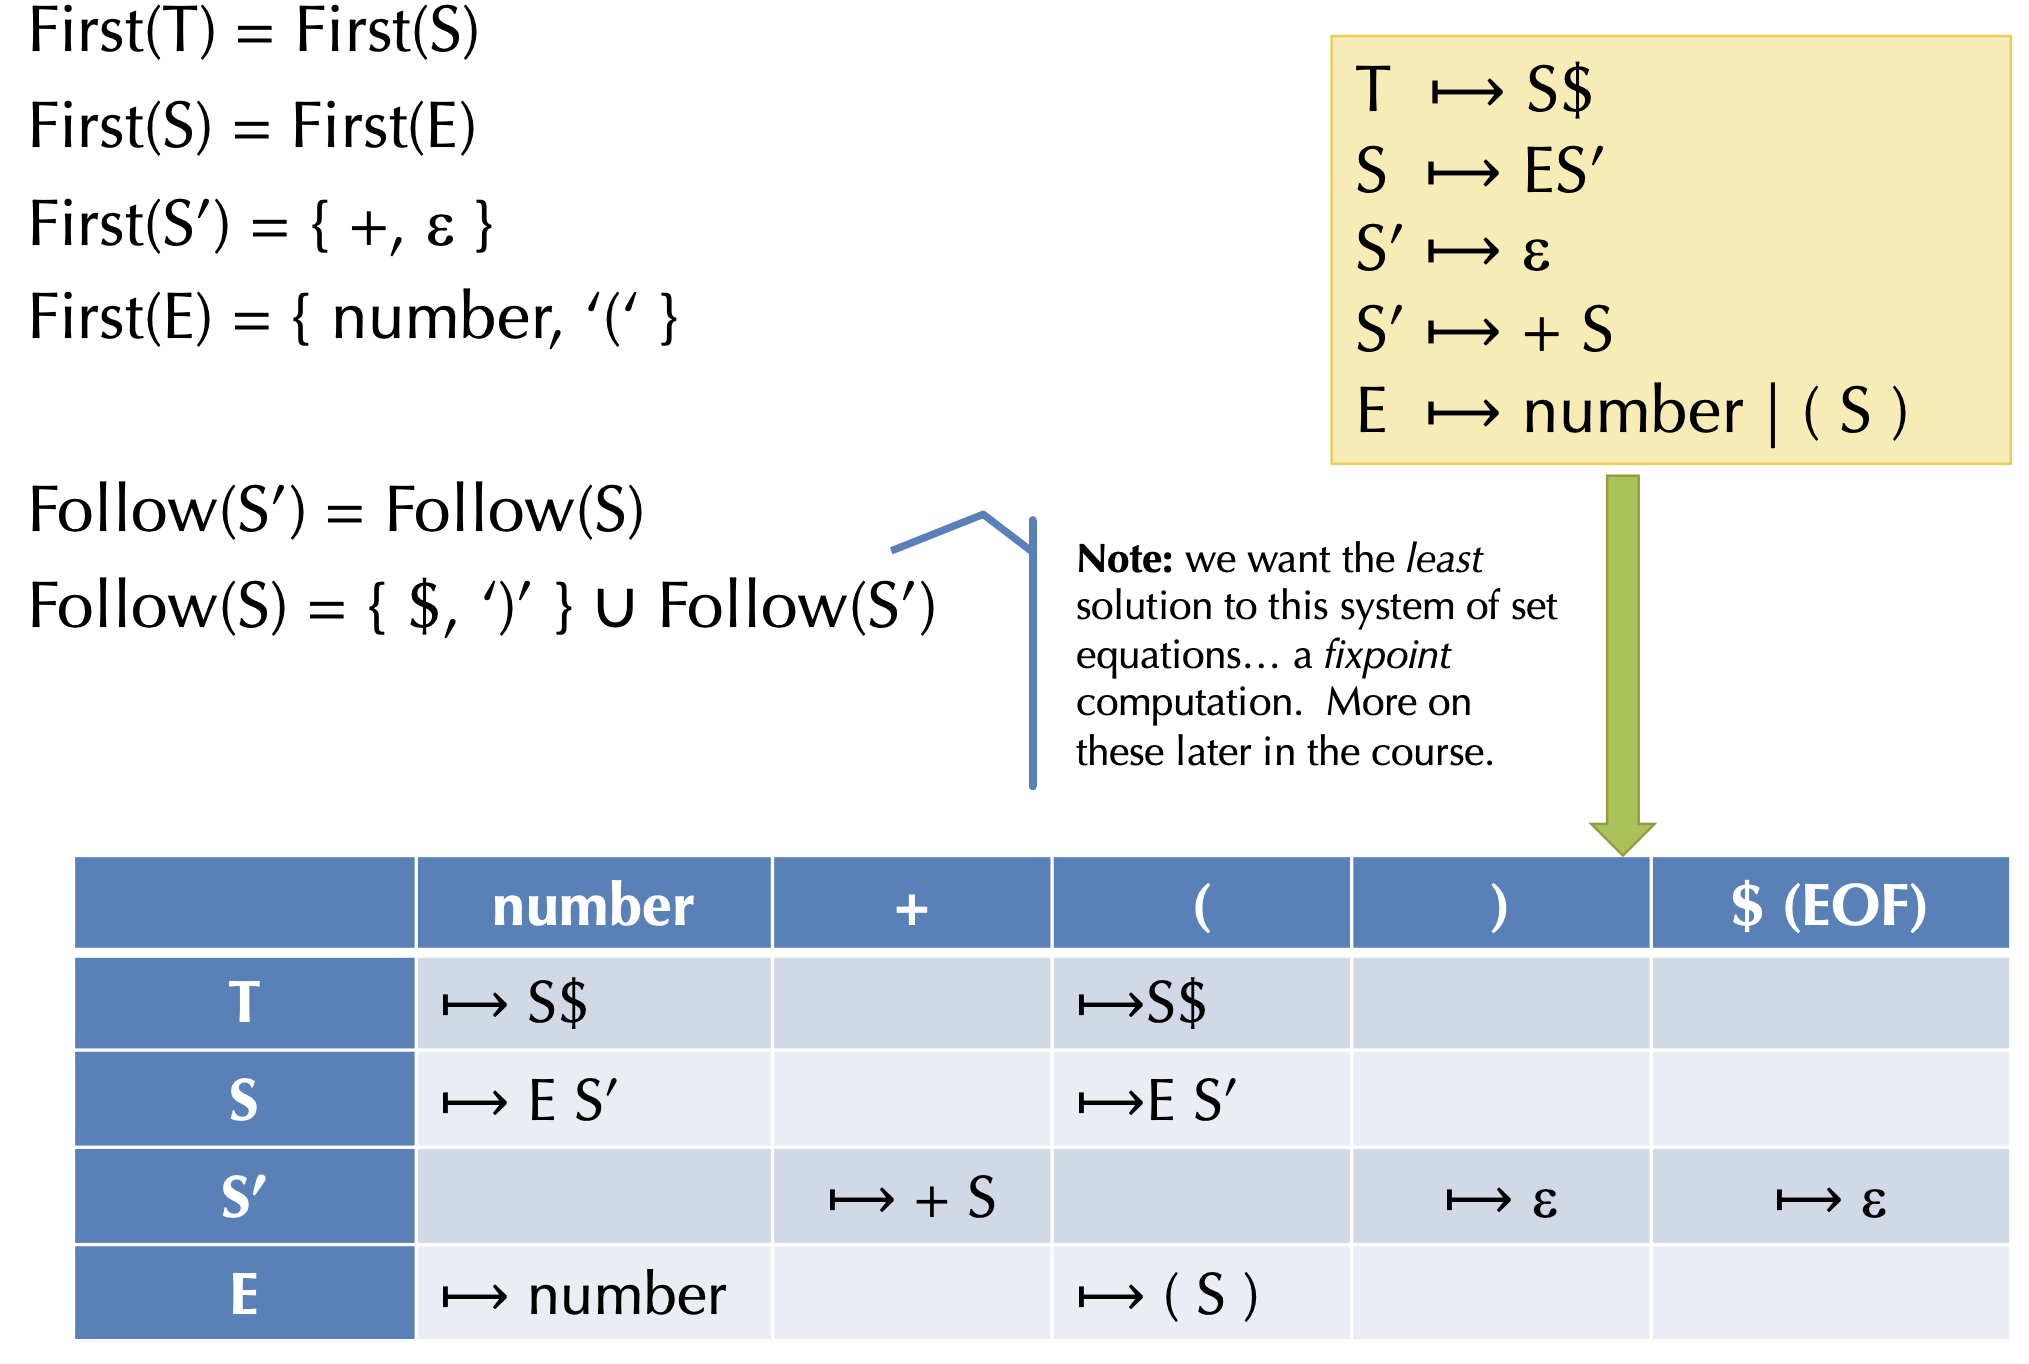
\includegraphics[width=\linewidth]{assets/ll1.png}
\end{center}

This can be extended to LL($k$) grammars by generating a bigger table.


\subsection*{LR Grammars and Bottom-Up Parsing}

LR grammars are more expressive than LL grammars. They can handle left-recursive and right-recursive grammars. However error reporting is poorer. \medskip

Bottom-up parsing is a sequence of \textbf{shift} and \textbf{reduce} operations:
\begin{itemize}
	\item Shift: Move look-ahead token to stack.
	
	\item Reduce: Replace symbols $\gamma$ at the top of the stack with nonterminal $X$ such that $X \to \gamma$ is a production. Pop $\gamma$, push $X$.
\end{itemize}

The parser state is made up of a stack of nonterminals and terminals, as well as the so far unconsumed input.\medskip
			
Action Selection Problem:
\begin{itemize}
	\item Given a stack $\sigma$ and a lookahead symbol $b$, should the parser \textbf{shift} $b$ onto the stack (new stack is $\sigma b$) , or \textbf{reduce} a production $X \mapsto \gamma$, assuming that $\sigma = \alpha \gamma$?
	
	\item Sometimes the parser can reduce, but should not, sometimes the stack can be reduced in different ways.
\end{itemize}

We want to decide based on a prefix $\alpha$ of the stack and the look-ahead. \medskip
		
In LR(0) we have states: items to track progress on possible upcoming reductions. An item is a production with an extra separator "." in the RHS. \medskip
		
The idea is that the stuff before the "." is already on the stack and the rest is what might be seen next. \medskip
		
Constructing the DFA:
\begin{itemize}
	\item Add new production: $S' \to S\$$, this is the start of the DFA.
						
	\item Add all productions whose LHS occurs in an item in the state just after the dot. Note that these items can cause more items to be added until a fixpoint is reached.
			
	\item Add transitions for each possible next (non-)terminal. Shift the dot by one in each of those states.
	
	\item Every state that ends in a dot is a reduce state.
\end{itemize} 

The parser then runs the DFA.\medskip

Instead of running the DFA from start for each step, we can store the state with each symbol on the stack - representing the DFA as a table of shape \texttt{state} $\times$ (\texttt{terminals} + \texttt{nonterminals}). \medskip

An LR(0) machine only works if states with reduce actions have a single reduce action else we will encounter shift/reduce or reduce/reduce conflicts (use LR(1) grammar). \medskip

In LR(1), each item is an LR(0) item plus a set of look-ahead symbols $A -\to \alpa . \beta, \; \mathcal L$. \medskip

To form the LR(1) closure, we first do the same as for LR(0). Additionally for each item $C \to .\gamma$ we add due to a rule $A \to \beta . C \gamma, \; \mathcal L$, we compute its look-ahead set $\mathcal M$ including FIRST($\gamma$) and if $\gamma$ can derive $\epsilon$ also $\mathcal L$. \medskip

\begin{center}
	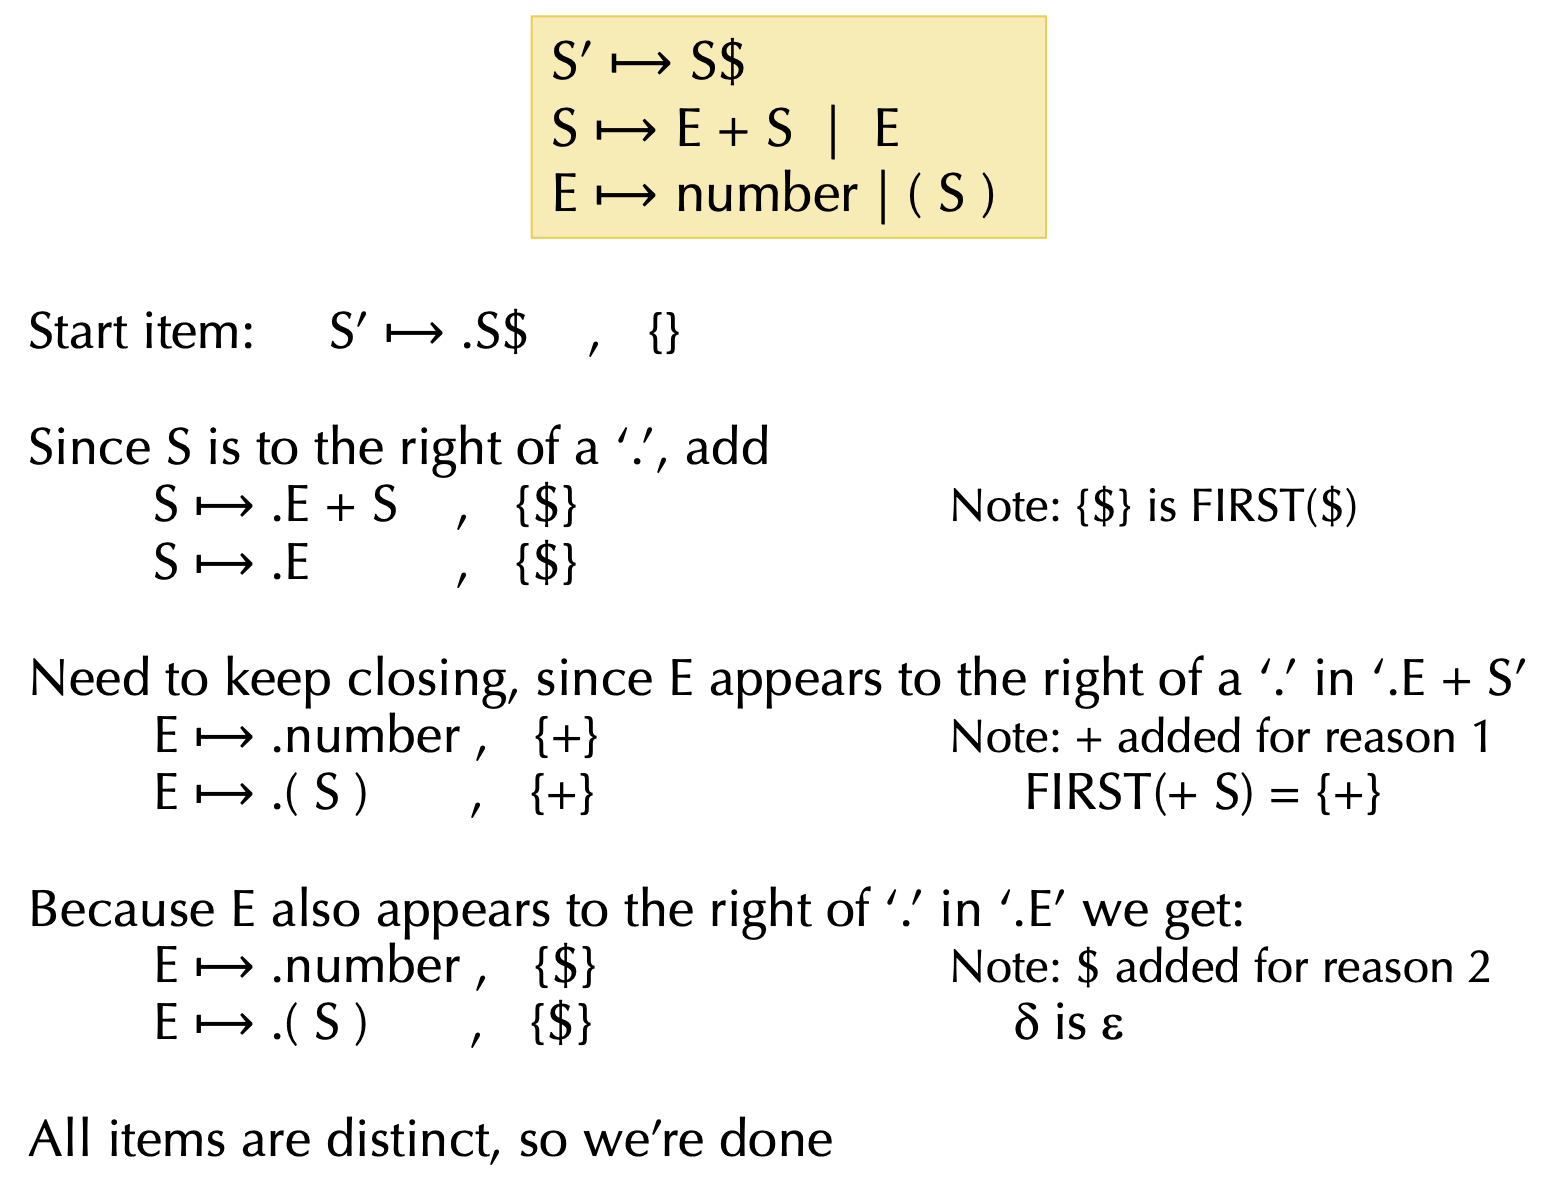
\includegraphics[width=\linewidth]{assets/lr1.png}
\end{center}
		
For LR(1) we have a shift-reduce conflict if the shifted token is contained in the follow set of the reduction.



\tikzset{every picture/.style={line width=0.8pt}} %set default line width to 0.75pt 

\begin{center}
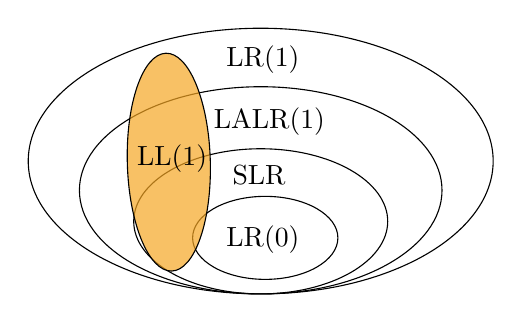
\begin{tikzpicture}[x=0.75pt,y=0.75pt,yscale=-1, xscale=1]
%uncomment if require: \path (0,719); %set diagram left start at 0, and has height of 719

%Shape: Ellipse [id:dp342446435028968] 
\draw   (505,130) .. controls (505,118.95) and (520.67,110) .. (540,110) .. controls (559.33,110) and (575,118.95) .. (575,130) .. controls (575,141.05) and (559.33,150) .. (540,150) .. controls (520.67,150) and (505,141.05) .. (505,130) -- cycle ;
%Shape: Ellipse [id:dp31528986086353894] 
\draw   (476.63,122.04) .. controls (476.63,102.73) and (504.02,87.07) .. (537.81,87.07) .. controls (571.61,87.07) and (599,102.73) .. (599,122.04) .. controls (599,141.35) and (571.61,157) .. (537.81,157) .. controls (504.02,157) and (476.63,141.35) .. (476.63,122.04) -- cycle ;
%Shape: Ellipse [id:dp8349221817367837] 
\draw   (450.47,107.09) .. controls (450.47,79.52) and (489.57,57.18) .. (537.81,57.18) .. controls (586.05,57.18) and (625.16,79.52) .. (625.16,107.09) .. controls (625.16,134.65) and (586.05,157) .. (537.81,157) .. controls (489.57,157) and (450.47,134.65) .. (450.47,107.09) -- cycle ;
%Shape: Ellipse [id:dp22985392220585588] 
\draw   (425.81,93) .. controls (425.81,57.65) and (475.96,29) .. (537.81,29) .. controls (599.67,29) and (649.81,57.65) .. (649.81,93) .. controls (649.81,128.35) and (599.67,157) .. (537.81,157) .. controls (475.96,157) and (425.81,128.35) .. (425.81,93) -- cycle ;
%Shape: Ellipse [id:dp012648097779113021] 
\draw  [fill={rgb, 255:red, 245; green, 166; blue, 35 }  ,fill opacity=0.7 ] (492.16,41.05) .. controls (503.2,40.76) and (512.77,64.01) .. (513.53,92.99) .. controls (514.3,121.97) and (505.96,145.7) .. (494.92,145.99) .. controls (483.88,146.28) and (474.31,123.02) .. (473.55,94.05) .. controls (472.78,65.07) and (481.11,41.34) .. (492.16,41.05) -- cycle ;

% Text Node
\draw (520,123) node [anchor=north west][inner sep=0.75pt]   [align=left] {LR(0)};
% Text Node
\draw (523,94) node [anchor=north west][inner sep=0.75pt]   [align=left] {SLR};
% Text Node
\draw (514,66) node [anchor=north west][inner sep=0.75pt]   [align=left] {LALR(1)};
% Text Node
\draw (520,36) node [anchor=north west][inner sep=0.75pt]   [align=left] {LR(1)};
% Text Node
\draw (477, 84) node [anchor=north west][inner sep=0.75pt]   [align=left] {LL(1)};
\end{tikzpicture}
\end{center}

  \section*{Lambda Calculus}

\begin{itemize}
	\item Lambda calculus has variables, functions and function application. Instead of \texttt{(fun x -> e)} we write: $\lambda x. e$
	
	\item The only values are closed functions
	
	\item To substitute value $v$ for variable $x$ in expression $e$ we replace all free occurrences of $x$ in $e$ by $v$: $e\{v / x\}$
	
	\item Function application is  interpreted by substitution.
	
	\item In \texttt{fun y -> x + y}, \texttt{x} is said to be free and \texttt{y} is bound by \texttt{fun y}.
	\item A term without free variables is closed, else it is open.
	
	\item Two terms that differ only by consistent renaming of bound variables are alpha equivalent.
	\item To avoid accidently capturing a free variable by a substitution $e_1 \{e_2 / x\}$, we first pick an alpha equivalent version of $e_1$ such that the bound variables do not mention the free variables of $e_2$.
	
	\item Operational Semantics is a way to give meaning to a program (interpreter) using inference rules. $exp \Downarrow v$ means $exp$ evaluates to $v$.

	\item With inference rules we can build up derivation or proof trees. Leaves of the tree are axioms.
\end{itemize}

  \section*{Typing}

Applying a set of inference rules allows for type checking of a program. 

\begin{itemize}
	\item A well-typed program either terminates in a well-defined way, or it continues computing forever.
	
	\item If we view types as sets of values, there is a natural inclusion relation Pos $ \subseteq $ Int. This gives rise to a subtype relation P $<:$ Int and to a subtyping hierarchy.

	\item The LUB (least upper bound) is defined for two types $T_1 \vee T_2$.
	
	\item Soundness of a subtypinig rule = Matches subset relation of value set
	
	\item Argument type is contravariant (it is okay if a function takes more arguments), output type is covariant (it is okay if a function returns less arguments).
	$$\frac{S_1 <: T_1 \qquad T_2 <: S_2}{(T_1 -> T_2) <: (S_1 -> S_2)}$$

	\item Mutable structure are invariant: covariant / contravariant reference types are unsound.
		
	\item Structural vs. Nominal Typing - is type equality / subsumption defined by the structure or the name.
\end{itemize}

\subsection*{OAT Type System}
\begin{itemize}
	\item Primitive (non-reference) types: \texttt{int, bool}
	
	\item Definitely non-null reference types: \texttt{R} (named) mutable structs with width subtyping, \texttt{strings}, \texttt{arrays}
	
	\item Possibly-null reference types: \texttt{R?}
	
	\item Subtyping \texttt{R} $<:$ \texttt{R?}
\end{itemize}

  \section*{Compiling Objects}

The \textbf{dispatch problem} occurs when the same interface is implemented by multiple classes. In the client program, it may be necessary to dynamically choose witch implementation to use. In order to do this, object contain a pointer to a \textbf{dispatch vector} (vtable) with pointer to method code. \medskip

For extension / inheritance, the dispatch vector gets extended at the end.\medskip

For \textbf{multiple inheritance} there are different approaches:
\begin{compactitem}[$\quad\bullet$]
	\item Allow multiple DV tables (C++), choose which DV to use based on static types, casting requires runtime operations.

	\item Use a level of indirection: Map method identifiers to code pointers using a hash table, search up through the class hierarchy.

	\item Give up separate compilation: Use sparse dispatch vectors or binary decision trees.
\end{compactitem}

\textbf{Multiple Dispatch Vectors}: Objects may have multiple entry points with individual DVs, casts change entry point of a variable
\vspace{-8pt}
\begin{center}
	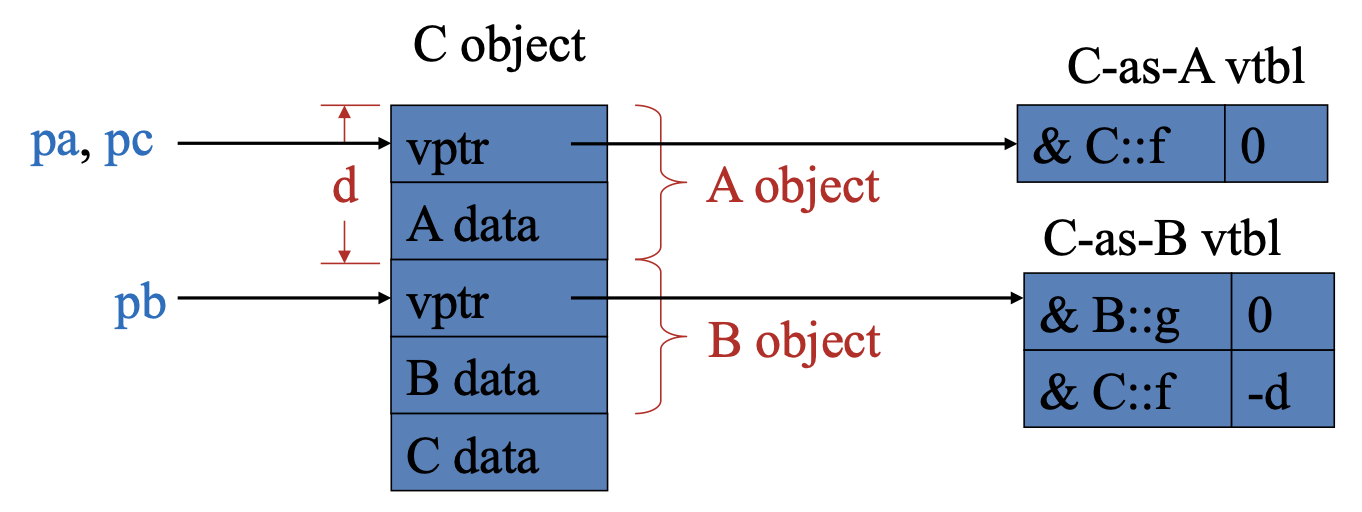
\includegraphics[width=0.7\linewidth]{vtable.png}
\end{center}
\vspace{-20pt}

  \section*{Optimizations}

There are different kinds of optimization: Power, Space, Time.

\begin{compactitem}[$\quad\bullet$]
	\item \textbf{Constant Folding}: If operands are statically known, compute value at compile-time. More general \textbf{algebraic simplification}: Use mathematical identities.

	\item \textbf{Constant Propagation}: If $x$ is a constant replace its uses by the constant.

	\item \textbf{Copy Propagation}: For $x = y$ replace uses of $x$ with $y$

	\item \textbf{Dead Code Elimination}: If side-effect free code can never be observed, safe to eliminate it.

	\item \textbf{Inlining}: Replace a function call with the body of the function (arguments are rewritten to local variables).

	\item \textbf{Code Specialization}: Create Specialized versions of a function that is called form different places with different arguments.

	\item \textbf{Common Subexpression Elimination}: It is the opposite of inlining, fold redundant computations together.

	\item \textbf{Loop Optimizations}
	\begin{compactitem}[$\quad\bullet$]
		\item Hot spots often occur in loops (esp. inner loops)
		\item Loop Invariant Code Motion (hoist outside)
		\item Strength Reduction (replace expensive ops by cheap ones by creating a dependent induction variable)
		\item Loop Unrolling
	\end{compactitem}
\end{compactitem}


\subsection*{Dataflow Analysis}

Almost every dataflow analysis is a variation of the following algorithm.\smallskip

\textbf{Forward Must Dataflow Analysis}
\begin{lstlisting}
	for all n, in[n] = T, out[n] = T
	repeat until no change in 'in' or 'out'
		for all n
			in[n] = intersect out[n`] for all n` in pred[n]
			out[n] = gen[n] union (in[n] \ kill[n])	
\end{lstlisting}
\textbf{Backward}: swap \texttt{in} and \texttt{out} and \texttt{pred} with \texttt{succ}.

\textbf{May}: swap $\top$ with $\bot$ or $\emptyset$ and replace \textcolor{blue}{\texttt{intersect}} with \textcolor{blue}{\texttt{union}}.\medskip

For each dataflow analysis we only need to define the set \texttt{gen}, \texttt{kill} as well as the domain of dataflow values $\mathcal L$ and a combining operator $\cup$ or $\cap$.\medskip

\textbf{Liveness} (Backward, May)\medskip

We can use the same registers for multiple \texttt{\%uids} if they are not alive at the same time
(\textbf{live[n]} = uids used before end/reassign).
We define \texttt{gen[s]} as all the variables used (RHS) and \texttt{kill[s]} as all the variables defined by statement $s$ (LHS). $\mathcal L$ corresponds to the variables and the combination operator to the set union.\medskip

It holds: in[$n$] $\supseteq$ gen[$n$], in[$n$] $\supseteq$ out[$n$] $\backslash$ kill[$n$] and out[$n$] $\supseteq$ in[$n'$] if $n' \in $ succ[$n$].\medskip

\textbf{Reaching Definition} (Forward, May)\medskip

What variable definitions reach a particular use of a variable? Used for constant and copy propagation.
\texttt{in / out} is the set of nodes defining some variable such that the definition may reach the beginning resp.
end of the current node. For a statement $d_i: A=B:$ we have $d_i \in \textbf{gen[n]}$ and $\textbf{kill[n]}=\{d_i | \text{$d_i$ defines A (LHS)} \;\backslash\; gen[n]$ (inclusive of previous nodes) \medskip

It holds: out[$n$] $\supseteq$ gen[$n$], in[$n$] $\supseteq$ out[$n'$] if $n' \in$ pred[$n$] and out[$n$] $\supseteq$ in[$n$] $\backslash$ kill[$n$] or out[$n$] $\cup$ kill[$n$] $\supseteq$ in[$n$].\medskip

\textbf{Available Expressions} (Forward, Must)\medskip

Used for common subexpression elimination.
\texttt{in / out} are the set of nodes whose values are available on entry / exit of the current node.
For a statement $d_i: A=B:$ we have $d_i \in \textbf{gen[n]} \;\backslash\; \text{kill[n]}$ and $\textbf{kill[n]}=\{d_i | \text{$d_i$ uses A (RHS)}\}$\medskip

\textbf{Very Busy} (Backward, Must)\medskip

An expression is very busy at location $p$, if every path from $p$ must evaluate the expression before any variable is redefined.
It is used for hoisting expressions. \textbf{in/out/gen allow for expressions (x+y)} \medskip

\texttt{gen[B]} = \{expr; expr a op b is evaluated in B, neither a nor b are subsequently redefinded in B \}\smallskip

\texttt{kill[B]} = \{expr; a or b of expr a op b are defined in B and a op b is not subsequently evaluated in B\} \medskip

\textbf{Dominators} (Forward, Must)\medskip

Define \texttt{dom[n]} as the set of all nodes that dominate \texttt{n}, i.e. \texttt{dom[n] = out[n]}, \texttt{gen} is the singelton set of the node itself, \texttt{kill} is the empty set.\medskip

The iterative solution computes the ideal meet-over-path solution if the flow function distributes over $\cap$. Most of the problems that express properties on how the program computes are distributive and compute the MOP solution, analyses of what the program computes do not (e.g. constant propagation). Our analyses also always terminate, as the flow function (\texttt{out[n] = ...}) is monotonic.\medskip

\textbf{Soundness} is defined as an under approximation of the set of variables.


\subsection*{Register Allocation}

\textbf{Linear-Scan Register Allocation}\medskip

Compute liveness information and then scan through the program, for each instruction try to find an available register, else spill it on the stack.\medskip

\textbf{Graph Coloring}\medskip

Compute liveness information for each temp, create an inference graph (nodes are temps and there is an edge if they are alive at the same time), try to color the graph.\medskip

\textbf{Kempe's Algorithm}:
\begin{compactitem}[$\quad\bullet$]
	\item Find a node with degree $< k$ and cut it out of the graph
	\item Recursively $k$-color the remaining subgraph
	\item When remaining graph is colored, there must be at least one free color available for the deleted node.
	\item If the graph cannot be colored we spill a node and try again.
\end{compactitem}\medskip

This can be improve by adding \texttt{move} related edges (temps used in a move should have the same color). More aggresively, we may coalesce two move-related nodes into one. This may increase the degree of a node, so we need to be careful. \medskip

\textbf{Brigg}'s strategy is to only coalesce if the resulting node has fewer than $k$ neighbors with degree $\geq k$. \medskip

\textbf{George}'s strategs is to only coalesce if for every neighbor $t$ of one of the coalescing nodes $x$, $t$ also interferes with the other coalescing node or $t$ has degree $< k$.\medskip

Precolored Nodes: Certain variables must be pre-assigned to registers (\texttt{call}, \texttt{imul}, caller-save registers)



\subsection*{Dominator Trees}

To identify loops in a CFG we use domination. $A$ dominates $B$ ($A$ dom $B$), if the only way to reach $B$ from start node is via $A$. This relation is transitive, reflexive and anti-symmetric. This can be computed as forward must dataflow analysis. $A$ strictly dominate $B$, if $A \neq B$ and $A$ dom $B$. The Hasse diagram of the dominates relation is called the \textbf{dominator tree}.\medskip

A loop is a set of nodes in the CFG, with a distinguished entry (header) and exit nodes. It is a strongly connected component (SSC), where every node is reachable from every other node. A loop contains at least 1 \textbf{back edge} (target dominates the source).\medskip

\textbf{How-to: Natural Loop}

For a back edge $s \rightarrow h$, $s=\text{source, }h=\text{header}$:
\begin{compactitem}[$\quad\bullet$]
	\item Look for all nodes dominated by your header (dominates itself)
	\item From these, take the ones which you can use to reach $s$ without going through $h$
	\item Merge loops with the same header $h$
\end{compactitem}\smallskip

We can formally define a loop as:
$$L(s \to h) = \{ n' \; | \; s \text{ is reachable from } n' \text{ in } G
	\backslash\{h\}  \} \cup \{h\}$$

\vspace{3pt}
The \textbf{dominance frontier} of a node $A$ is the set of all CFG nodes
$\gamma$ such that $A$ dominates a predecessor of $\gamma$, but does not
strictly dominate $\gamma$. Intuitively: starting at $A$, there is a path to $\gamma$, but there is another route that does not go through $A$. It is the set of nodes where $A$'s dominance stops. \medskip

\textbf{How-to: Dominance Frontier}

For each node $X$: All neighbor nodes it can get to that have some other way to get there
are part of DF[$X$]. Then do the same for any nodes dominated by $X$ and add them all
to DF[$X$].\medskip

\textbf{How-to: Least Fixed Point} of \textbf{Join Points}

$J[N] = DF_k[N] \text{ where } DF_0 = DF[N];\; DF_{i+1}[N] = DF[DF_i[N] \cup N]$

\begin{minipage}{\columnwidth} % very dirty, but it works to prevent random column break

	To determine the join points (places where $\phi$-nodes have to be inserted)
	for $N = \{X,Y\}$:
	\begin{compactitem}[$\quad\bullet$]
		\item Find $DF_0[N] = DF[\{X,Y\}] = \{A\} \quad(DF[X] \cup DF[Y] \cup \ldots)$
		\item Find $DF_1[N] = DF[\{X, Y, A\}] = \{Y,A,B\}$
		\item Continue until: $DF_2[N] = DF[\textcolor{blue}{\{X,Y,A,B\}}] = \textcolor{blue}{\{X,Y,A,B\}}$
		\item These are our \textbf{join points}: $J[N] = DF_2[N] = \{X,Y,A,B,C\}$
	\end{compactitem}

	\subsection*{Single Static Assignment (SSA)}
\end{minipage}

Each LLVM IR \texttt{\%uid} can be assigned only once. When coming from an \texttt{if-else} branch or similar, we might not know which \texttt{\%uid} to take. That's where we introduce $\phi$-nodes.\medskip

A $\phi$-node picks the version of a variable depending on the label from which the $\phi$-node was entered. It even allows usage of later-defined \texttt{\%uid}s.\medskip

\begin{lstlisting}
	%uid = phi <type> v1, <label1>, ..., vn, <labeln>
\end{lstlisting}\medskip

Converting to SSA:
\begin{compactitem}[$\quad\bullet$]
	\item Start with CFG with \texttt{alloca}s, identify promotable \texttt{alloca}s
	\item Compute dominator tree information
	\item Calculate \texttt{def} / \texttt{use} information for each variable
	\item Insert $\phi$-nodes at necessary join points
	\item Replace \texttt{load} / \texttt{stores} with freshly generated \texttt{\%uid}s
	\item Eliminate unneeded \texttt{alloca}s
\end{compactitem}\medskip


Some \texttt{alloca}s are needed, either if the address of the variable is taken or the address escapes by being passed to a function. If neither condition holds, it is promotable.\medskip

Necessary join points are defined as the transitive closure of the dominance frontier of all nodes where a variable $x$ is defined or modified. Then we just need to pick the value of $x$ depending on the predecessors of the node where we just inserted the $\phi$-node.\medskip

To place $\phi$-nodes without breaking SSA, we insert \texttt{load}s at the end of each block, and insert \texttt{store}s after $\phi$-nodes. We can then optimize load after stores (LAS) by substituting all uses of the load by the value stored and remove the load itself. Then, we can eliminate dead \texttt{stores} and dead \texttt{alloca}s. At the very end, we can eliminate $\phi$-nodes with only a single value, or identical values from each predecessor.

  \section*{Garbage Collection}

An object \texttt{x} is \textbf{reachable} iff a register contains a pointer to \texttt{x} or another reachable object \texttt{y} contains a pointer to \texttt{x} (we also consider the stack as a source for pointers!). If an object is not reachable, we might want to consider it as garbage. \medskip

Reachable objects can be found by starting from registers and following all pointers. \medskip

\textbf{Mark and Sweep} \smallskip

When memory runs out, GC executes two phases: \textbf{mark phase}: trace reachable objects; \textbf{sweep phase}: collects garbage objects (extra bit reserved for memory management)\medskip

One problem is that it only runs when we are out of memory - yet we need memory
to keep track of our todo-list (not yet checked pointers). The solution to this
is \textbf{pointer reversal}. Pointer reversal enables a DFS
of the reachable objects without using additional memory. We keep only a
backward and forward pointer. The \textbf{forward pointer (FP)} points to next object to
be examined. The \textbf{backward pointer (BP)} points to the
one we just handled.
Each iteration we go along a pointer ($\text{P} \to new$): Set $\text{P} \to \text{BP}$,
$\text{BP} \to cur$ and $\text{FP} \to new$.

When going back in reverse, we point the original pointer back to its original node.
\medskip

\textbf{Pros}: Objects stay in place, no need to update pointers. \textbf{Cons}: Fragmentation.\medskip

\textbf{Stop and Copy} \smallskip

Memory is organized into two areas: \textbf{Old space} (used for allocation), \textbf{new space} (use as a reserve for GC). \medskip

When old space is full all reachable objects are moved to the new space and the roles of the spaces are swapped. To avoid copying twice, a already copied object is replaced by a forwarding pointer to the new copy. \medskip

To achieve this without extra space, we divide the new space in three regions: copied and scanned, a scan pointer followed by the copied region, and the alloc pointer followed by the empty region. We copy the objects pointed to by roots, then, as long as scan hasn't caught up to alloc: Find each object pointed to by the object at scan, if it's a forwarding pointer update our current pointer, if not, copy the pointed-to object to the new space, update alloc pointer, and update our current pointer. Increment the scan pointer. \medskip

Despite having to update many pointers, stop and copy is generally the fastest GC technique, as allocation and collection is relatively cheap when there's lots of garbage.


Stop and Copy moves objects around. Pointers to those objects must also be updated. However, objects (structs) in C and C++ do not carry any metadata that identify which members are pointers and therefore it is impossible to properly update them.\medskip

\textbf{Reference Counting }\smallskip

Store number of references in the object itself, assignments modify that number. If the reference count is zero, free the object. Cannot collect circular structures and updating the reference count on each assignment is slow.

  \section*{Exercises}

\hrulefill

\textbf{Ex.} In parsing, ...
\begin{compactitem}[$\quad\bullet$]
	\item[$\square$] LL(1) parsers are more powerful than LR(0) parsers.
	\item[$\boxtimes$] LR(1) parsers are more powerful than LL(1) parsers.
	\item[$\boxtimes$] LALR(1) may introduce new reduce/reduce conflicts compared to LR(1) when parsing the same grammar.
	\item[$\square$] LALR(1) may introduce new shift/reduce conflicts compared to LR(1) when parsing the same grammar.
\end{compactitem}

\hrulefill

\textbf{Ex.} For context free grammars, ...
\begin{compactitem}[$\quad\bullet$]
	\item[$\boxtimes$] LR parsers can handle left-recursive grammars.
	\item[$\boxtimes$] LR parsers can handle right-recursive grammars.
	\item[$\square$] LL parsers can handle left-recursive grammars.
	\item[$\square$] LR(0) parsers are more powerful than LL(1) parsers.
	\item[$\boxtimes$] even with an unambiguous CFG, there may be more than one derivation.
\end{compactitem}

\hrulefill

\textbf{Ex.} A left-recursive grammar cannot be implemented by an LL(k) parser for any k.
$$ \boxtimes \text{ True } \qquad \square \text{ False }$$

\hrulefill

\textbf{Ex.} LR(k) grammars cannot be right recursive.
$$ \square \text{ True } \qquad \boxtimes \text{ False }$$


\hrulefill

\textbf{Ex.} There is no such thing as a shift/shift conflict for a LR parser.
$$ \boxtimes \text{ True } \qquad \square \text{ False }$$


\hrulefill

\textbf{Ex.} Calling conventions, ...
\begin{compactitem}[$\quad\bullet$]
	\item[$\boxtimes$] specify where arguments and return values should be stored.
	\item[$\square$] specify the starting address of stack and heap.
	\item[$\boxtimes$] can be disregarded by the compiler for functions that are not exposed to external callers as an optimization.
\end{compactitem}

\hrulefill

\textbf{Ex.} Any type-safe program, ...
\begin{compactitem}
	\item[$\boxtimes$] can raise en exception.
	\item[$\square$] can treat non-code values as code.
	\item[$\square$] always terminates.
	\item[$\boxtimes$] can raise a segfault (unsure).
\end{compactitem}

\hrulefill

\textbf{Ex.} Nominal subtyping, ...
\begin{compactitem}[$\quad\bullet$]
	\item[$\boxtimes$] requires us to explicitly declare subtyping relationships.
	\item[$\square$] is used by OAT for struct subtyping.
	\item[$\square$] is a subcategory of structural subtyping.
	\item[$\boxtimes$] is used by Java for subtyping.
\end{compactitem}

\hrulefill

\textbf{Ex.} A basic block, ...
\begin{compactitem}[$\quad\bullet$]
	\item[$\boxtimes$] starts with a label.
	\item[$\square$] can contain more than one control-flow instruction.
	\item[$\boxtimes$] is always executed starting from the basic block's first instruction.
\end{compactitem}

\hrulefill

\textbf{Ex.} Strength reduction, ...
\begin{compactitem}
	\item[$\square$] refers to a class of optimizations that can be profitably applied irrespective of the target architecture.
	\item[$\boxtimes$] is applicable to loops, by creating a dependent induction variable.
	\item[$\square$] can only be meaningfully applied if the IR on which the optimization is applied is in SSA form.
	\item[$\square$] reduces the static number of operations that are performed.
\end{compactitem}

\hrulefill

\textbf{Ex.} Which of the following are examples of forward analysis?
\begin{compactitem}
	\item[$\square$] Liveness analysis
	\item[$\boxtimes$] Available expressions
	\item[$\boxtimes$] Available registers
\end{compactitem}

\hrulefill

\textbf{Ex.} Which of the following statements are true?
\begin{compactitem}
	\item[$\square$] Contradictory to its name, the linear scan register allocation runs in a log-linear time in the number of program variables.
	\item[$\square$] Spilling two registers is always less efficient than spilling one.
	\item[$\square$] To apply linear scan register allocation, we need to compute the reaching definitions and the liveness analysis.
\end{compactitem}

\hrulefill

\textbf{Ex.} Consider the following dominance frontier DF of a graph:
DF[$ U $] = $\{ Y \}$,
DF[$ V $] = $\{ Z, W, Y \}$,
DF[$ W $] = $\{ V, Y \}$,
DF[$ X $] = $\{  \}$,
DF[$ Y $] = $\{ V \}$,
DF[$ Z $] = $\{  \}$.
There is a variable $x$ that is modified at nodes $N = \{X, Y, Z\}$. Determine all nodes
where $\phi$ functions for $x$ have to be inserted, i.e., the join points for $N$ with respect to $x$.
Determine the least fixed point of the sequence:
$$J[N] = \text{DF}_k[N] \text{ where } \text{DF}_0[N] = \text{DF}[N]; \text{DF}_{i+1}[N] = \text{DF}[\text{DF}_i[N] \cup \{N\}]$$\smallskip

$\text{DF}_0[\{X, Y, Z\}] = \{V\}$,

$\text{DF}_1[\{X, Y, Z, V\}] = \{V, W, Z, Y\}$,

$\text{DF}_1[\{V, W, Z, Y\}] = \{V, W, Z, Y\} = J[\{X, Y, Z\}]$

\hrulefill

\textbf{Ex.} What are the types of the followint \texttt{getelementptr} instructions?
\begin{lstlisting}
	struct B {
		int64_t c;
		struct B *d;
		struct A e[10][10];
	}; 
\end{lstlisting}

\texttt{getelementptr \%struct.B* @g, i64 0} : \textcolor{blue}{\texttt{struct.B*}}

\texttt{getelementptr \%struct.B* @g, i64 0, i64 0} : \textcolor{blue}{\texttt{i64*}}

\texttt{gep \%struct.B* @g, i64 0, i64 2, i64 5} : \textcolor{blue}{\texttt{[10 x struct.A]*}}

\hrulefill

\textbf{Ex.} If we try to precolor nodes in an inference graph while adhering to the calling convention, what problem might we face?\medskip

The problem is that multiple return values and arguments that interfere with each other must use the same registers.

\hrulefill

\textbf{Ex.} Apply Mark and Sweep:

\vspace{-11pt}
\begin{center}
	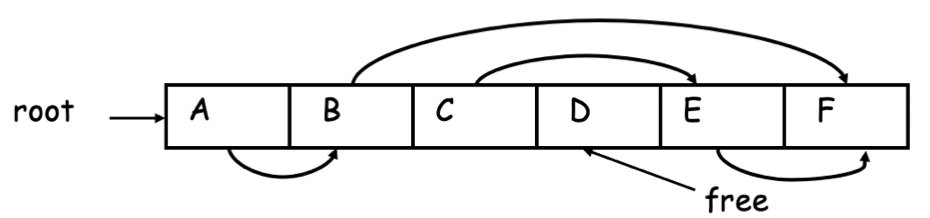
\includegraphics[width=0.5\linewidth]{before_ms.png}
\end{center}

\begin{multicols*}{2}
	After Mark:

	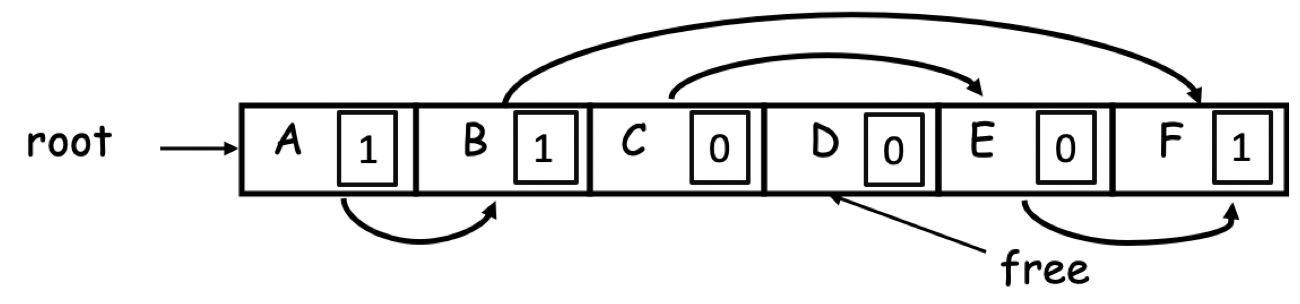
\includegraphics[width=\linewidth]{mark.png}

	After Sweep:

	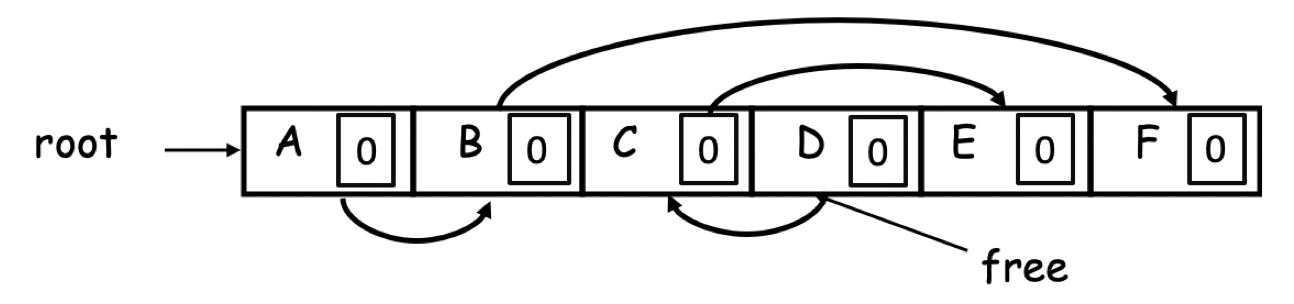
\includegraphics[width=\linewidth]{sweep.png}
\end{multicols*}

\hrulefill

\textbf{Ex.} Apply Stop and Copy:
\begin{multicols*}{2}
	Before:

	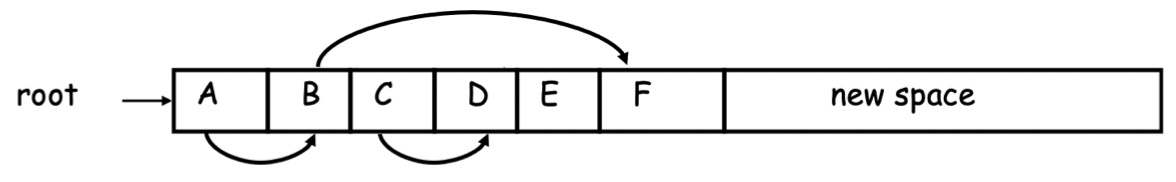
\includegraphics[width=\linewidth]{before_sc.png}
	\columnbreak

	After:
	\vspace{-11pt}

	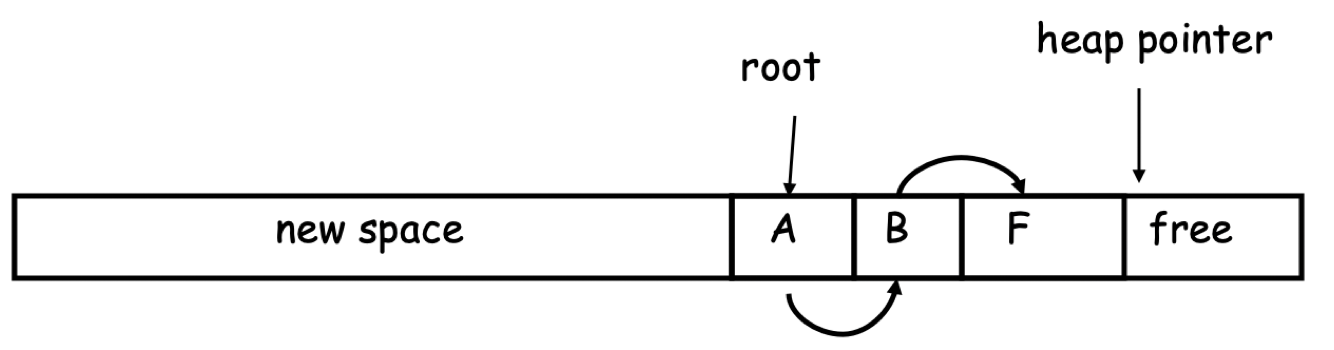
\includegraphics[width=\linewidth]{after_sc.png}
\end{multicols*}


  %\begin{center}
  %  
\includegraphics[width=0.7\linewidth]{you_can_do_it.jpg}
  %\end{center}

\end{multicols*}
\end{document}

% ____ FOOTER ______________________________________________________
% Content and Template: 
% original by Danny Camenisch (dcamenisch@inf.ethz.ch), 2023
% based on different summaries from many helpful people
